\documentclass{article}
\usepackage{graphicx}
\graphicspath{ {./nastran_figs/} }
\title{Acoustic Cavities in Nastran 95}
\author{Excerpts from NASA Nastran Manuals}
\date{November 2020}

\begin{document}

\maketitle

\section{User's Guide Information}

\subsection{2.4.3 Acoustic Cavity Analysis}

An acoustic cavity analysis may be performed with Rigid Format 3 to obtain,
the stationary waves in the steady-state flow of a gas through an axisym-
metric chamber with radial slots. The width and depth of the slots and the
diameter of the center volume may vary along the axis of the chamber. The
boundaries of the chamber are assumed to be rigid. The output available
includes pressures at points in the grid and the velocities in the fluid
elements.


\subsection{7.2.3 Acoustic Cavity Analysis}

The acoustic cavity analysis capability was implemented primarily to obtain
the resonant frequencies of a compressible fluid in a solid rocket motor
cavity. The enclosed gas is modeled with finite elements. The surrounding
propellant is assumed to be rigid and small motion theory is used, i.e., the
steady state velocities are small with respect to the wave velocity. Rigid
Format 3 is used to obtain these resonant frequencies.

The spape of the cavity may consist of a circular center volume surrounded
by equally spaced narrow radial slots. The width and depth of the slots
and the diameter of the center volume may vary along the axis of the cav-
ity. The finite-element model is defined by a set of two-dimensional ele-
ments lying on the center plane of one slot and on the corresponding cross
section of the center yolume. The entire cavity is solved by assuming a
Fourier Series of pressure and velocity around the circumference.
With minor correction terms, the pressure coefficients in the slots couple di-
rectly with the Fourier coefficients of pressure in the center volume. The
user may request a printout of the pressures at the points and/or the ve-
locities in the elements.

Remarks:
\begin{itemize}
    \item The fluid grid points are defined by GRIDF cards for the
        central volume and by GRIDS cards for the slot area. One
        degree of freedom is produced for each point in the model.
        The width and number of slots are defined on the GRIDS card.
        If the slot point lies on the opening to the central cavity,
        the location is specified on a GRIDS card on which is also
        given a unique GRIDF identifier. This eliminates the need
        for inputting a separate GRIDF card for the same point. The
        SLBDY card is used to define a list of GRIDS points which
        lie on the opening to the central cavity. 
    \item The GRIDF points are connected by the CAXIF2, CAXIF3, and
        CAXIF4 elements. Each element defines a volume generated by
        revolving the cross section shape around the center axis.
        The CAXIF2 element defines a volume which contains the center
        axis.
    \item The GRIDS points are connected by the CSLOT3 and CSLOT4 ele-
        ments. Each element may have a different fluid property.
    \item The default properties of the model are defined by the re-
        quired AXSLOT card. The harmonic index N specifies the
        Fourier Series term to be analysed. N = 0 restricts the mo-
        tion to axisymmetric radial and longitudinal motion. N = 1
        defines the lateral motion where the velocity. is normal to
        the center axis, etc. Repeated runs with N = 0, 1, ..., M/2
        may be necessary to extract all possible modes. M is the
        number of radial slots specified.
    \item The default on all boundaries is a fixed surface. If a
        free surface with zero pressure is desired, the SPC or
        SPCl data cards may be used to constrain the pressure at
        selected points.
    \item The two dimensional wave equation problem may be solved
        by using only CSLOT elements and GRIDS points, by spec-
        ifying only one slot (M = 1) and by setting the harmonic
        index, N, to zero.
    \item The finite element approximation assumes that the veloc-
        ity is constant over the cross section of each element and
        that the pressure distribution does not vary across the
        width of the slot. In regions where the velocity may ab-
        ruptly change direction, a finer finite element mark
        should be chosen.
\end{itemize}

\subsection{7.2.3.1 Example - Acoustic Cavity Problem}

The acoustic cavity shown below consists of a central cavity having a radius
of four inches and four equally spaced slots. The cavity is open at the
right end. 'The slot width varies linearly with radial position. The input
data for the simple finite element model chosen is presented in Section
Three CSLOT elements and six CAXIF elements are used. The harmonic index
is one, which will result in lateral motion. That is, the gas will travel
back and forth across the cavity from one slot to the slot on the opposite
side.

Notes:
\begin{enumerate}
    \item The PRESSURE control card requests output pressures
        at the GRIDF and GRIDS points. the STRESS control
        card requests the velocities
        in the finite elements.
    \item Required for acoustic cavity analysis and defines the
        default density, compressibility, harmonic index, slot
        width, and number of slots for the overall problem.· .
        These values may be overridden by the individual cards
        below.
    \item Defines the points on the slot. GRIDS 2, 5, 8, 9 and 12
        also define GRIDF points 1, 4, 7, and 11 at the same
        location. The slot width is varied on these data cards.
    \item Defines remaining GRIDF points directly.
    \item Specifies the CSL0T elements, which, in this case use
        the default fluid properties and number of slots speci-
        fied on the AXSL0T card.
    \item Specifies the CAXIF elements of the central axisym-
        metric volume. The default fluid properties will be
        used.
    \item Identifies the GRIDS points at the interface between
        the slots and the central volume
    \item Sets the pressure at point 13 to zero.


\end{enumerate}

\begin{figure}[h]
    \centering
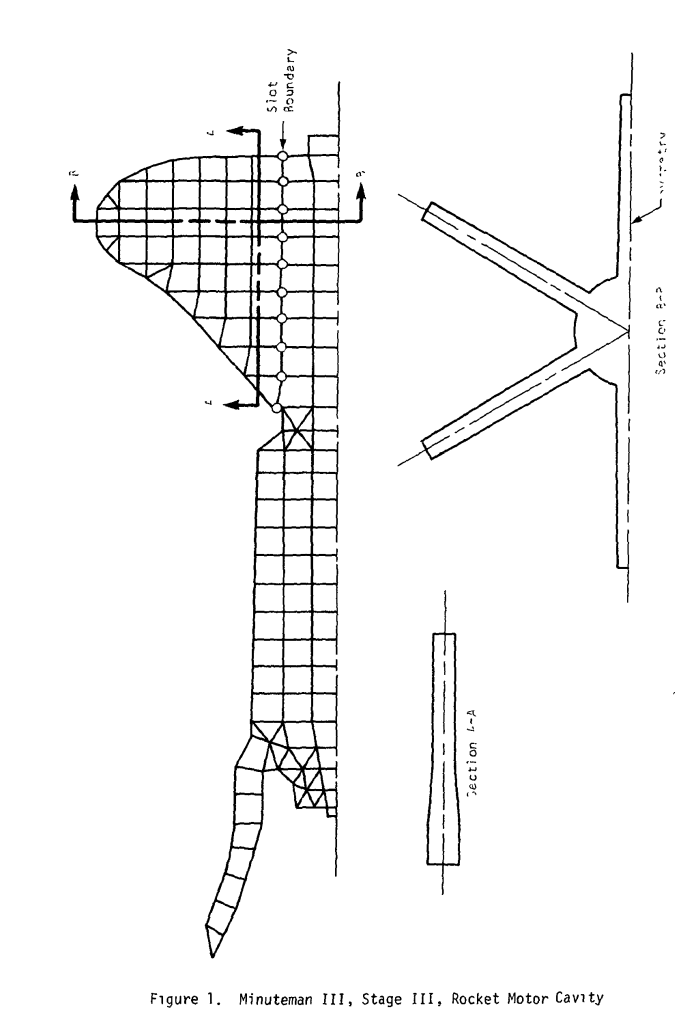
\includegraphics[scale=0.35]{nastran_fig1}
%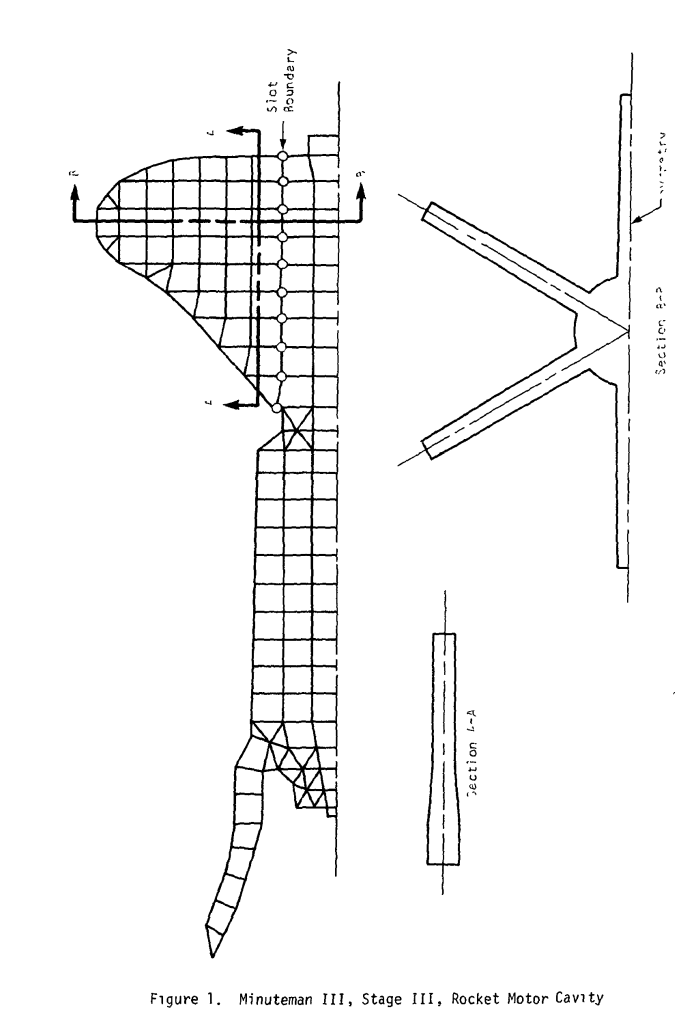
\includegraphics[width=3cm,height=5cm]{nastran_fig1}
    \caption{acoustic axisymmetric cavity analysis}
\end{figure}

\section{Demonstration Manual - Acoustic Cavity Analysis}


\subsection{A. Description}

This problem illustrates the use of NASTRAN to determine the acoustic modes in a cavity
containing both axisymmetric regions and evenly spaced radial slots. The solution is based
on an analogy between pressure and displacement, and between fluid particle acceleration and
internal structural force described in the Theoretical Manual.

\subsection{B. Input}

The finite element model for the motor cavity of the Minuteman III, Stage III, is shown in
Figure 1
As may be seen, it consists of six slots and a long, slender central cavity of
irregular shape. The model consists of AXIF2, AXIF3, and AXIF4 finite elements in the central
cavity, and SL0T3 and SL0T4 finite elements in the slotted region

\subsection{C. Results}

The vibration mode frequencies for harmonic n = 0 as determined with NASTRAN are shown in
Table 1. Also shown are the vibration mode frequencies as determined with an acoustic model
and reported in Reference 19.


\begin{figure}[v]
    \centering
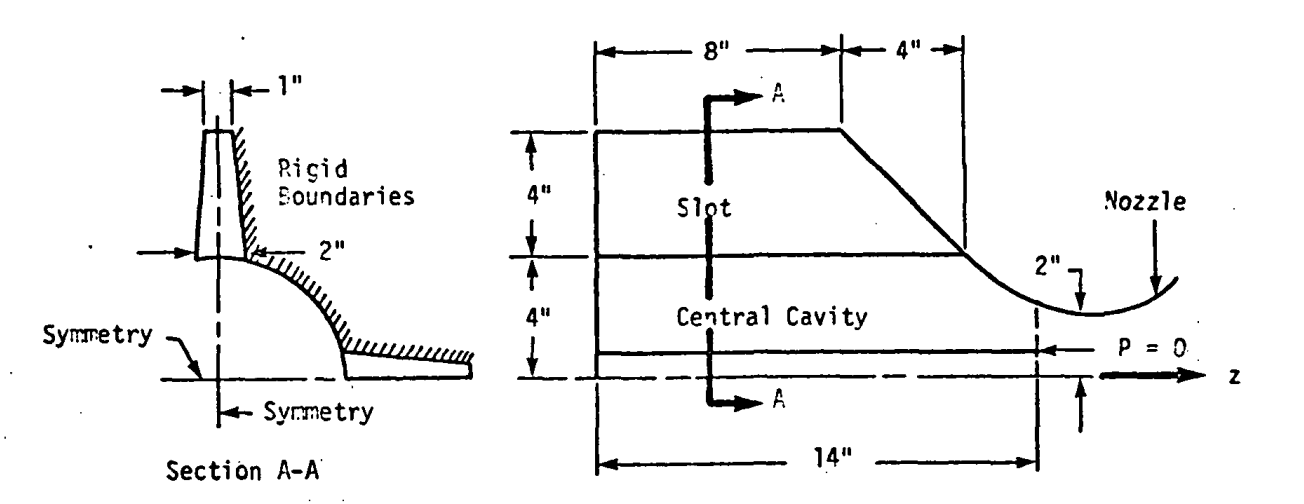
\includegraphics[scale=0.25]{nastran_fig2}
%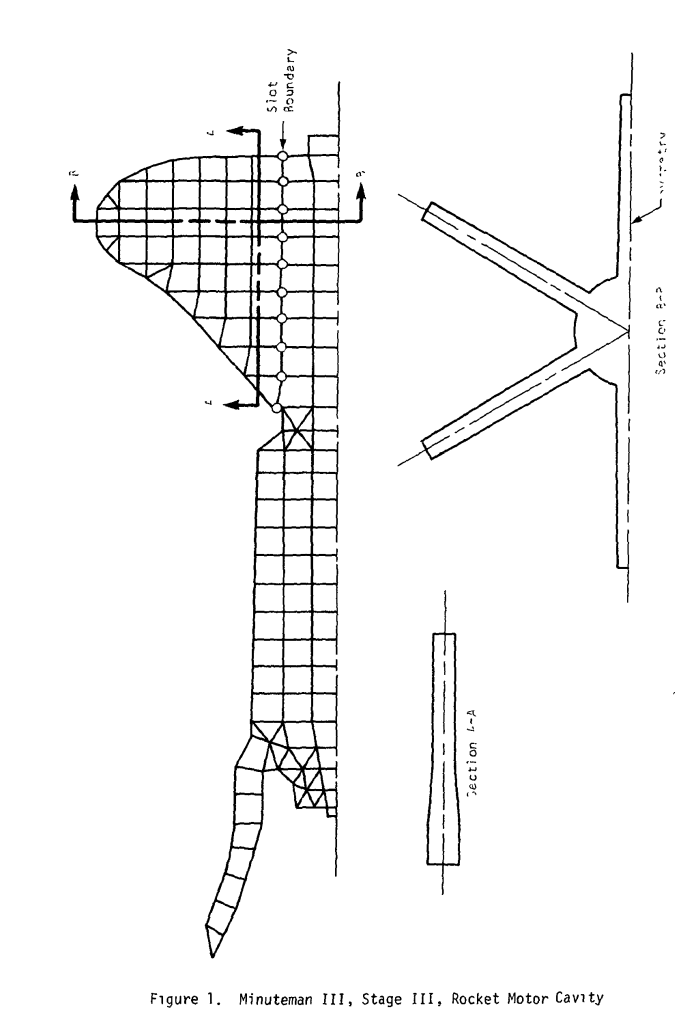
\includegraphics[width=3cm,height=5cm]{nastran_fig1}
    \caption{acoustic axisymmetric cavity analysis}
\end{figure}

\begin{figure}[v]
    \centering
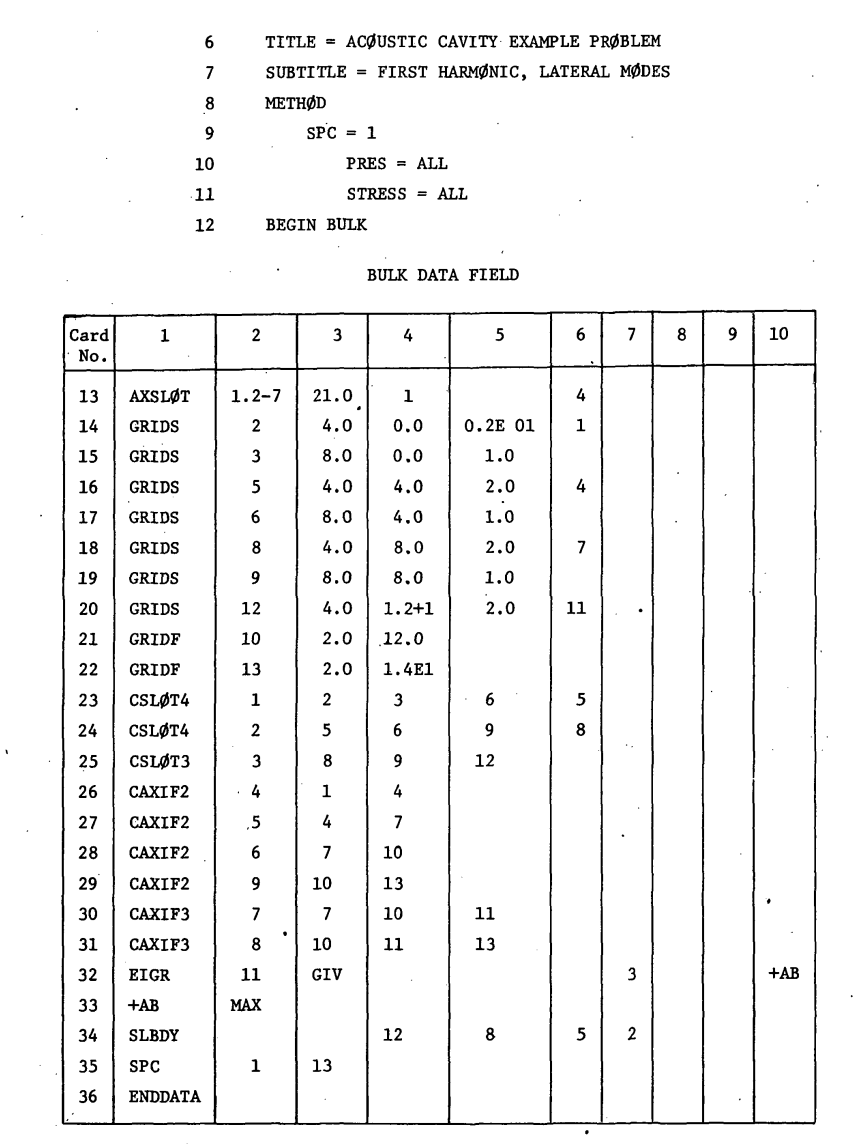
\includegraphics[scale=0.4]{nastran_fig3}
%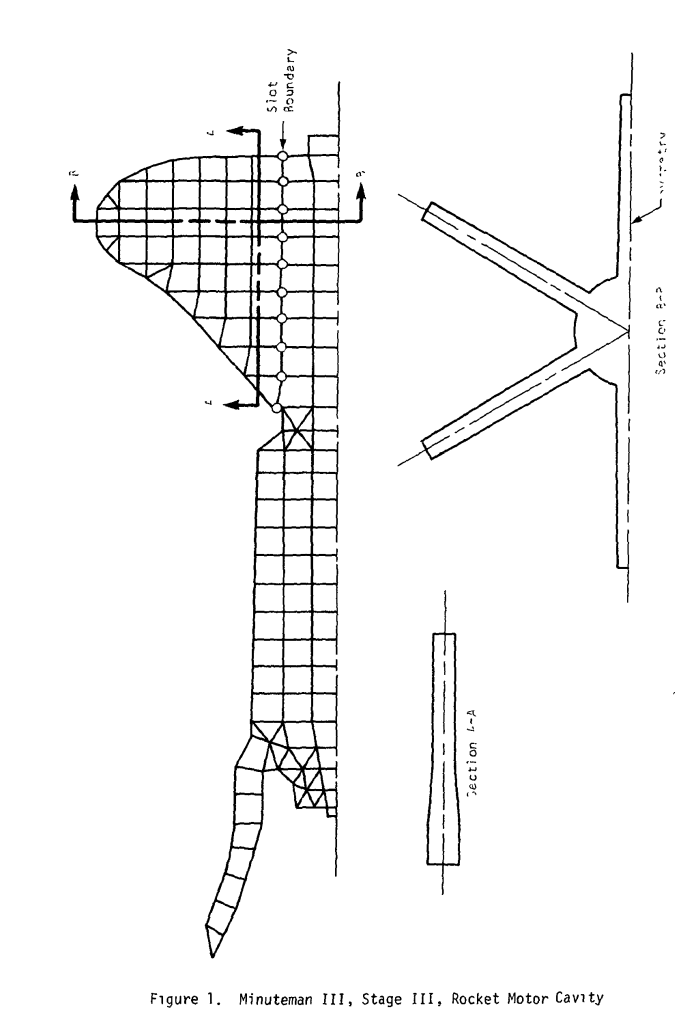
\includegraphics[width=3cm,height=5cm]{nastran_fig1}
    \caption{acoustic axisymmetric cavity analysis}
\end{figure}

\begin{figure}[h]
    \centering
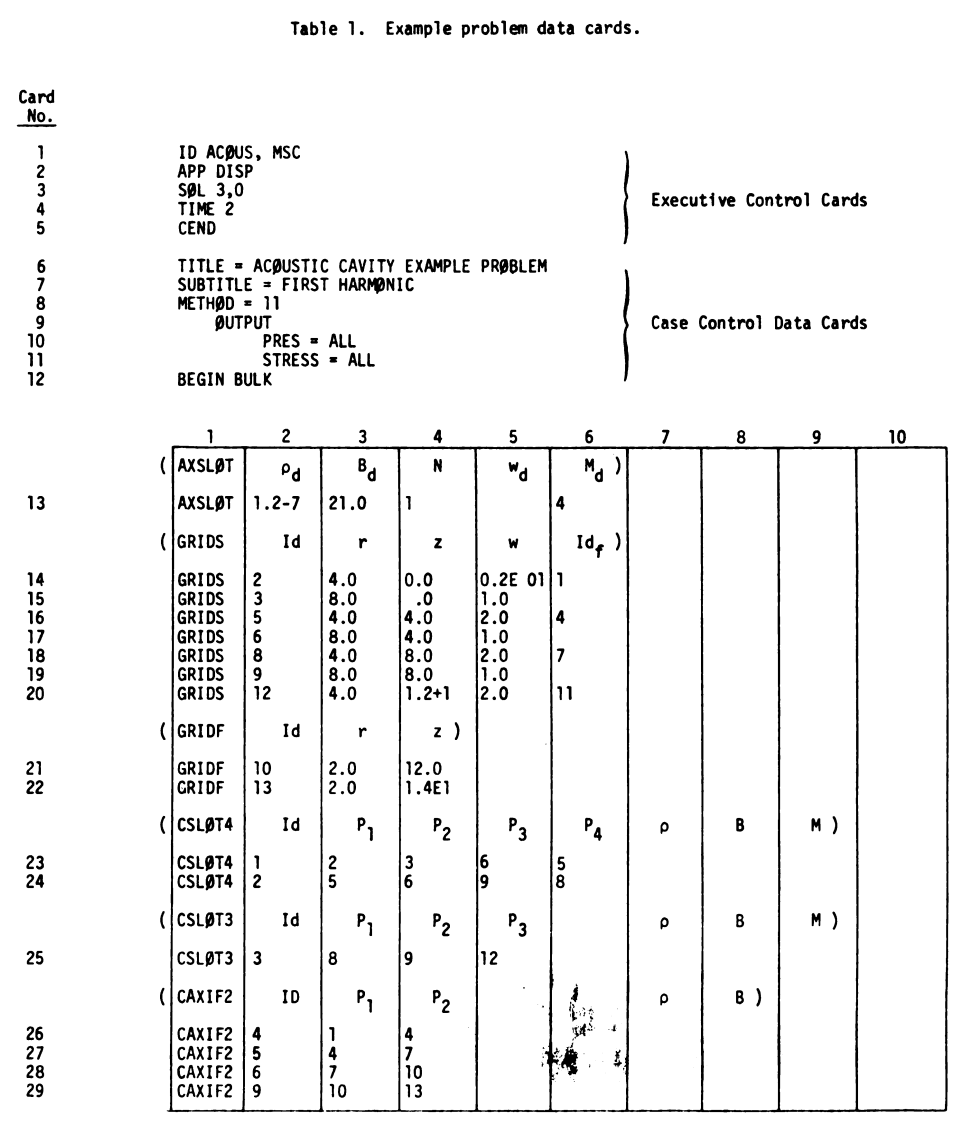
\includegraphics[scale=0.35]{nastran_fig4}
%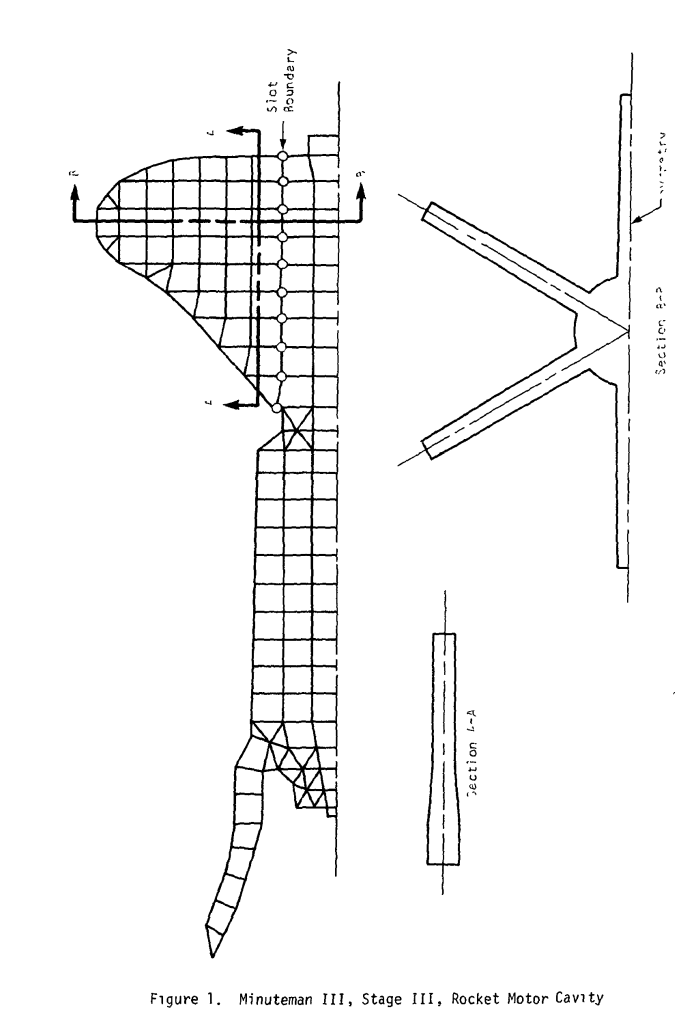
\includegraphics[width=3cm,height=5cm]{nastran_fig1}
    \caption{acoustic axisymmetric cavity analysis}
\end{figure}

\begin{figure}[h]
    \centering
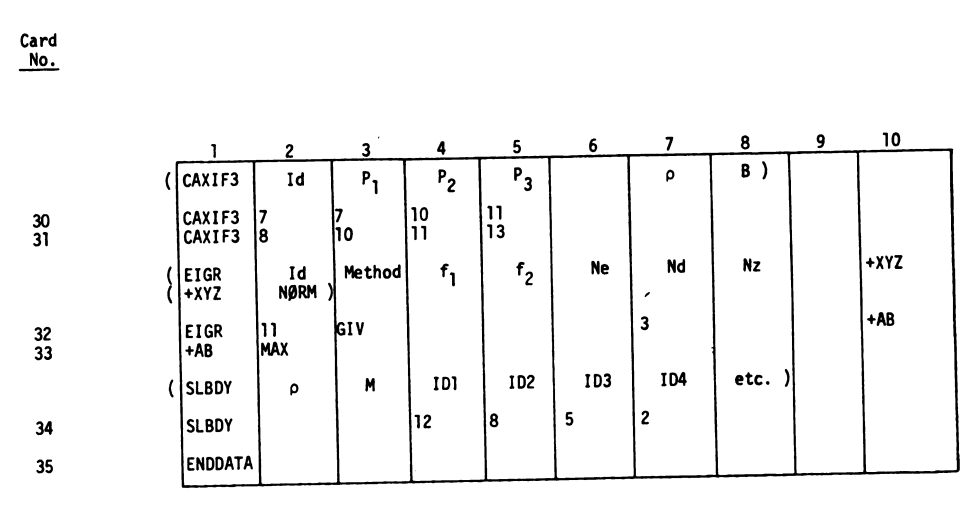
\includegraphics[scale=0.35]{nastran_fig5}
%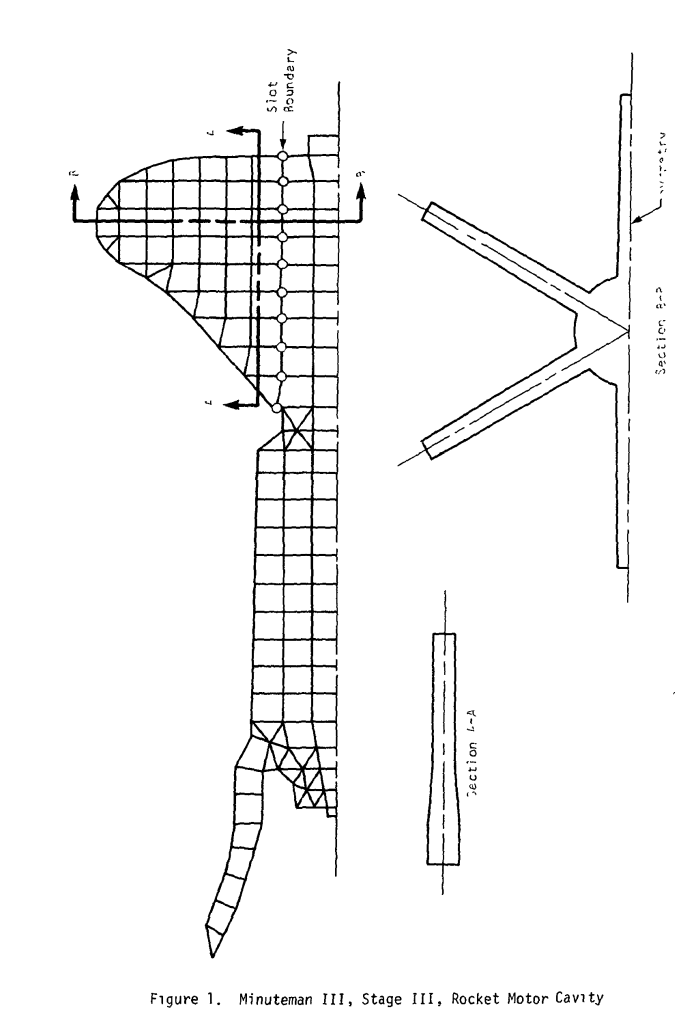
\includegraphics[width=3cm,height=5cm]{nastran_fig1}
    \caption{acoustic axisymmetric cavity analysis}
\end{figure}

\begin{figure}[h]
    \centering
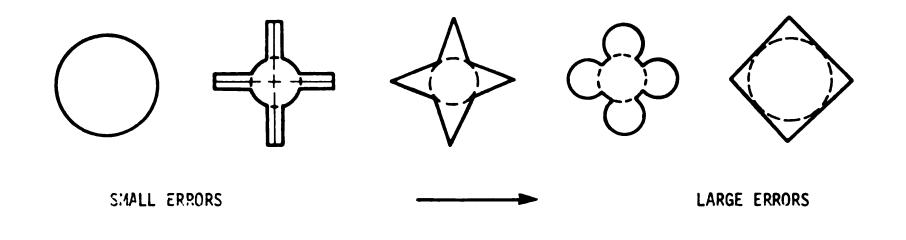
\includegraphics[scale=0.35]{nastran_fig6}
%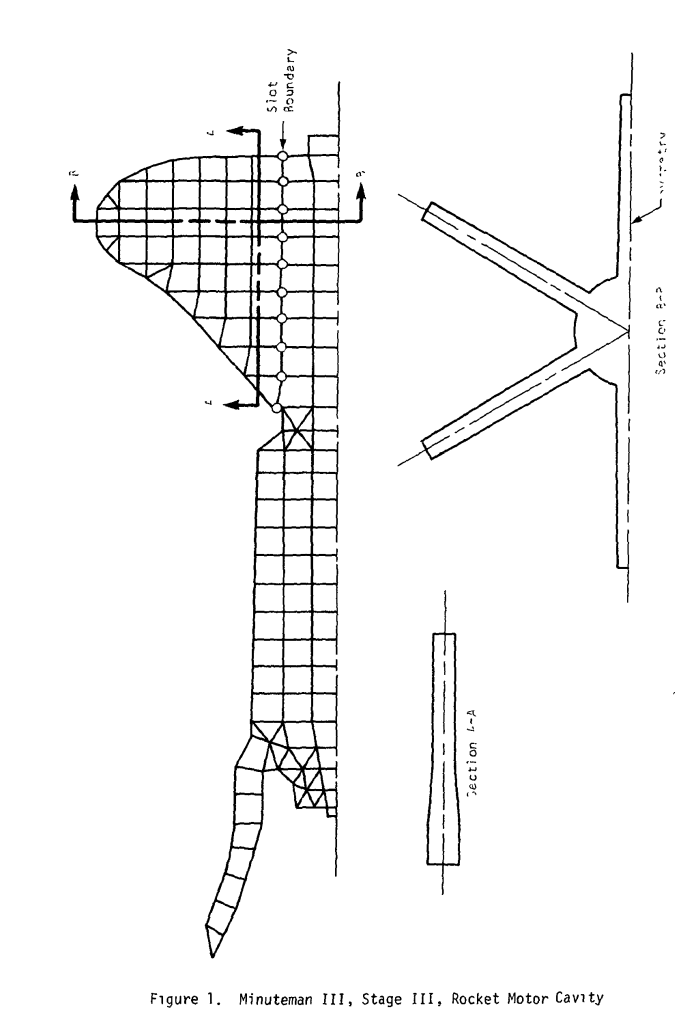
\includegraphics[width=3cm,height=5cm]{nastran_fig1}
    \caption{acoustic axisymmetric cavity analysis}
\end{figure}

\begin{figure}[h]
    \centering
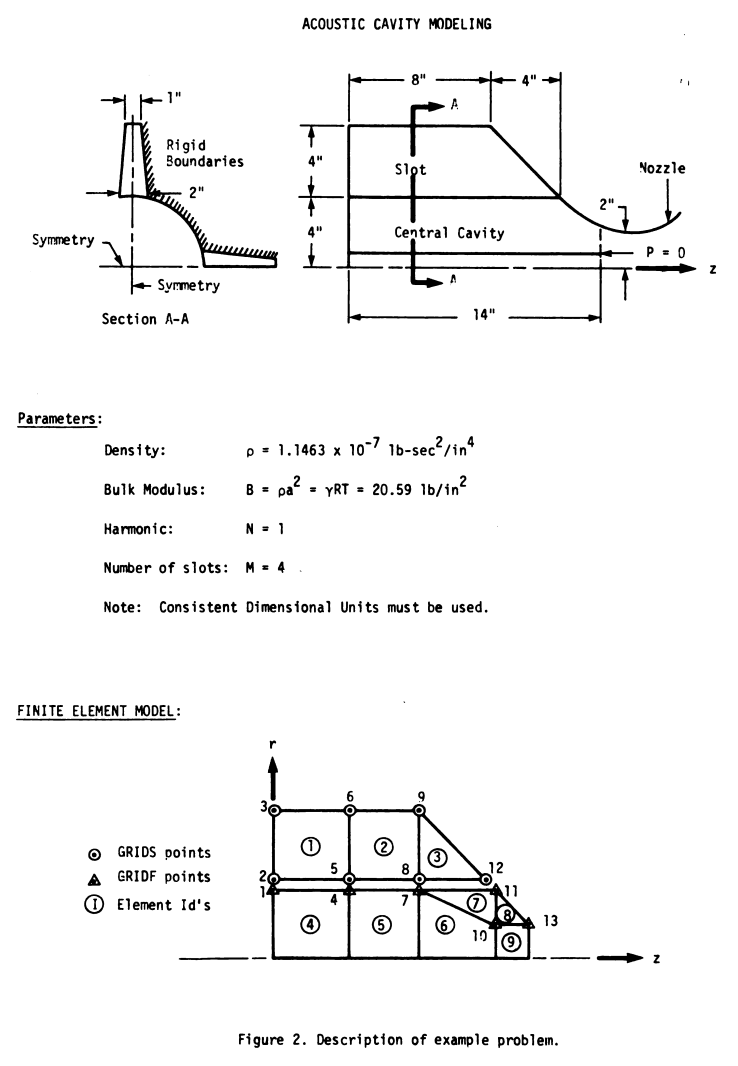
\includegraphics[scale=0.35]{nastran_fig7}
%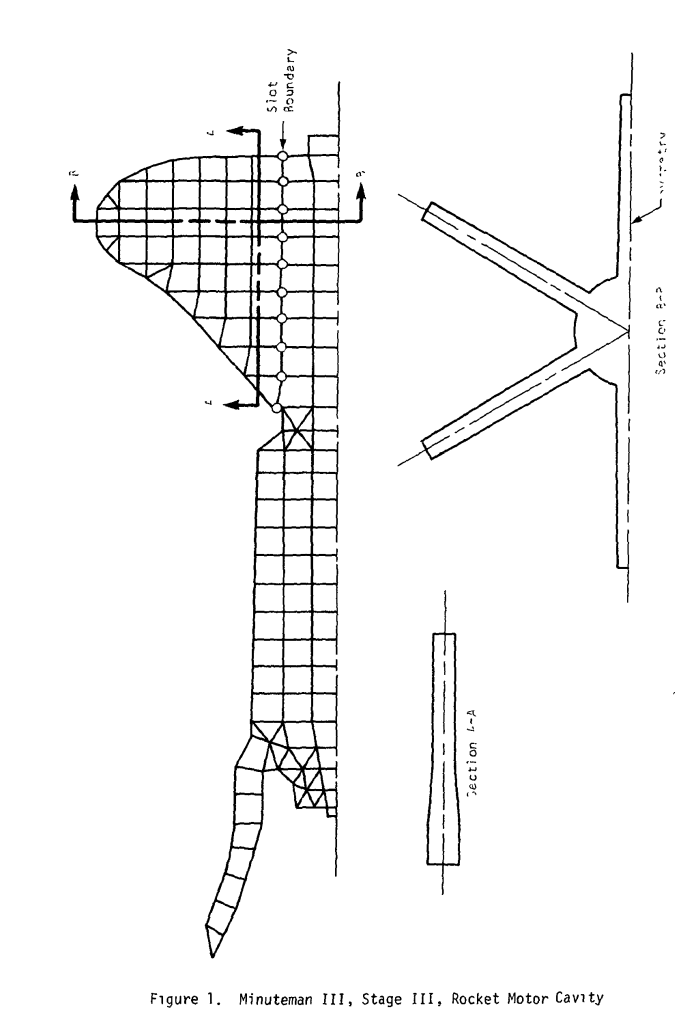
\includegraphics[width=3cm,height=5cm]{nastran_fig1}
    \caption{acoustic axisymmetric cavity analysis}
\end{figure}

\begin{figure}[h]
    \centering
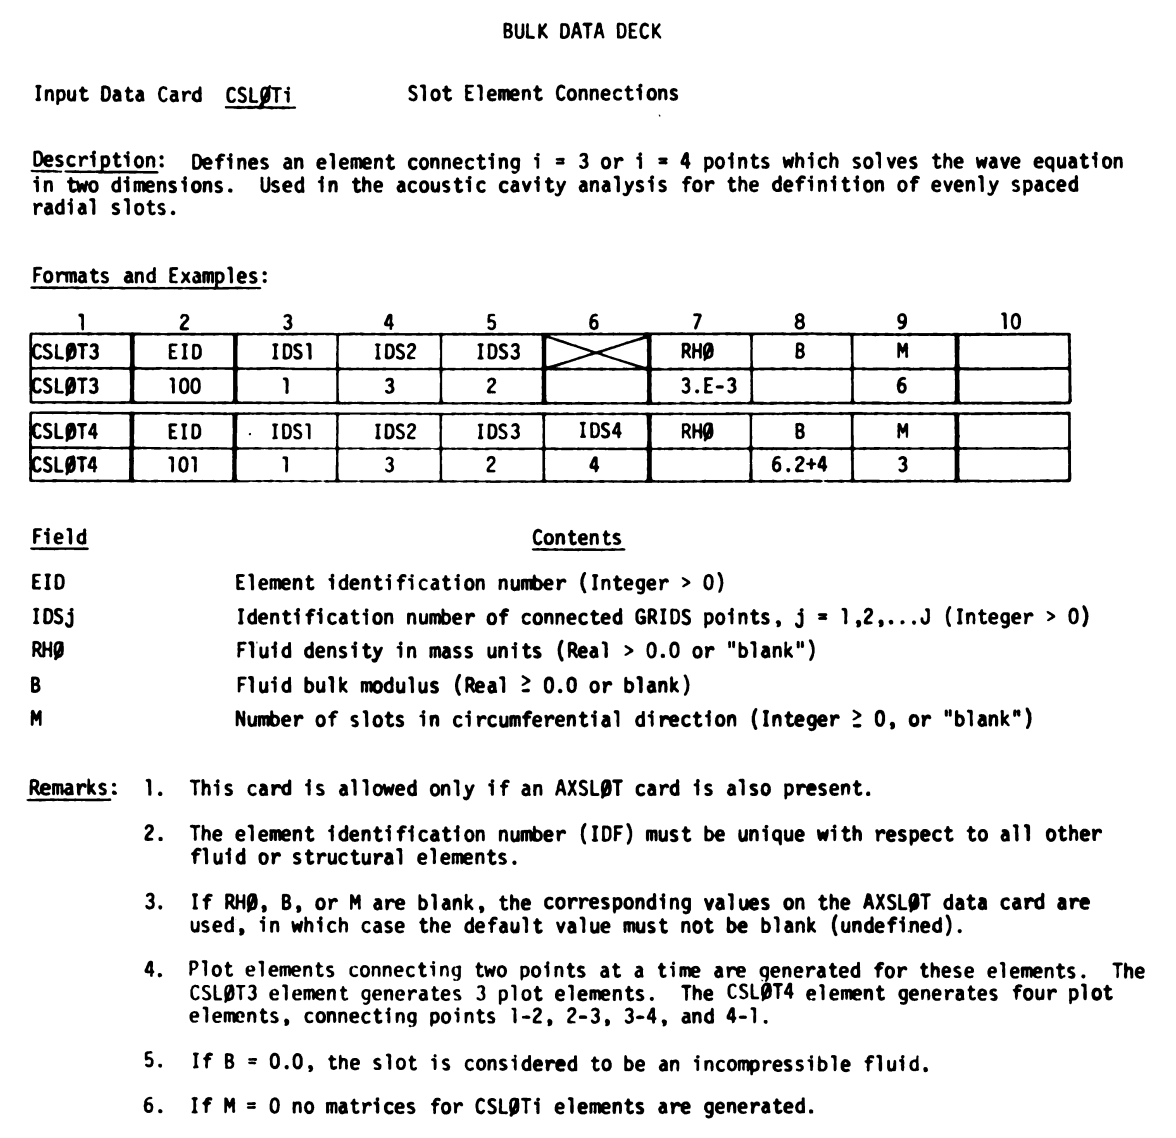
\includegraphics[scale=0.35]{nastran_fig8}
%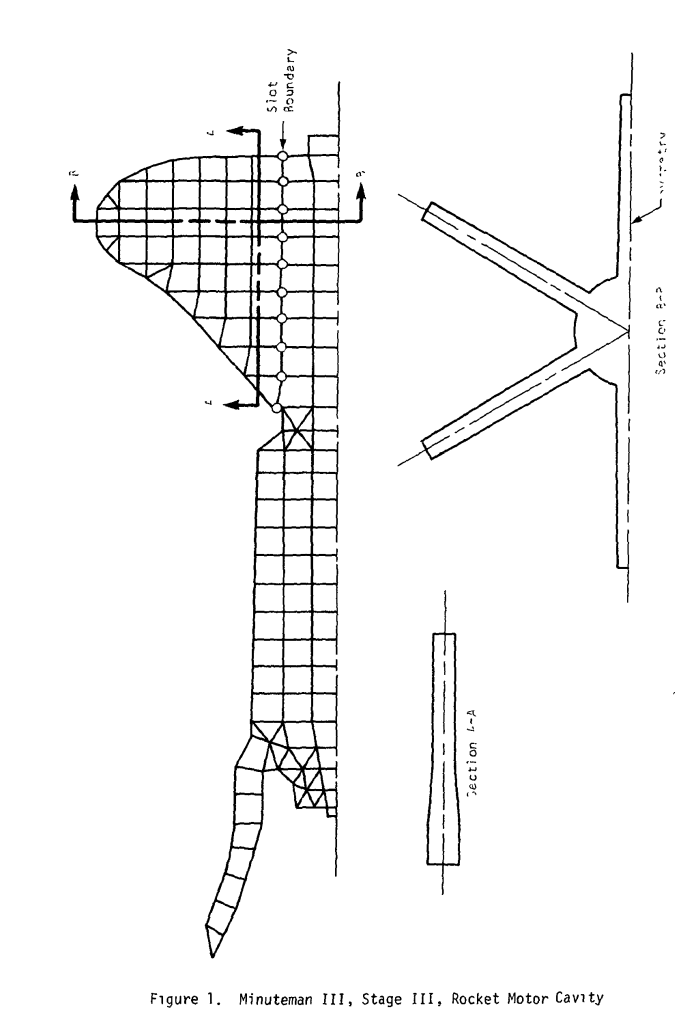
\includegraphics[width=3cm,height=5cm]{nastran_fig1}
    \caption{acoustic axisymmetric cavity analysis}
\end{figure}

\begin{figure}[h]
    \centering
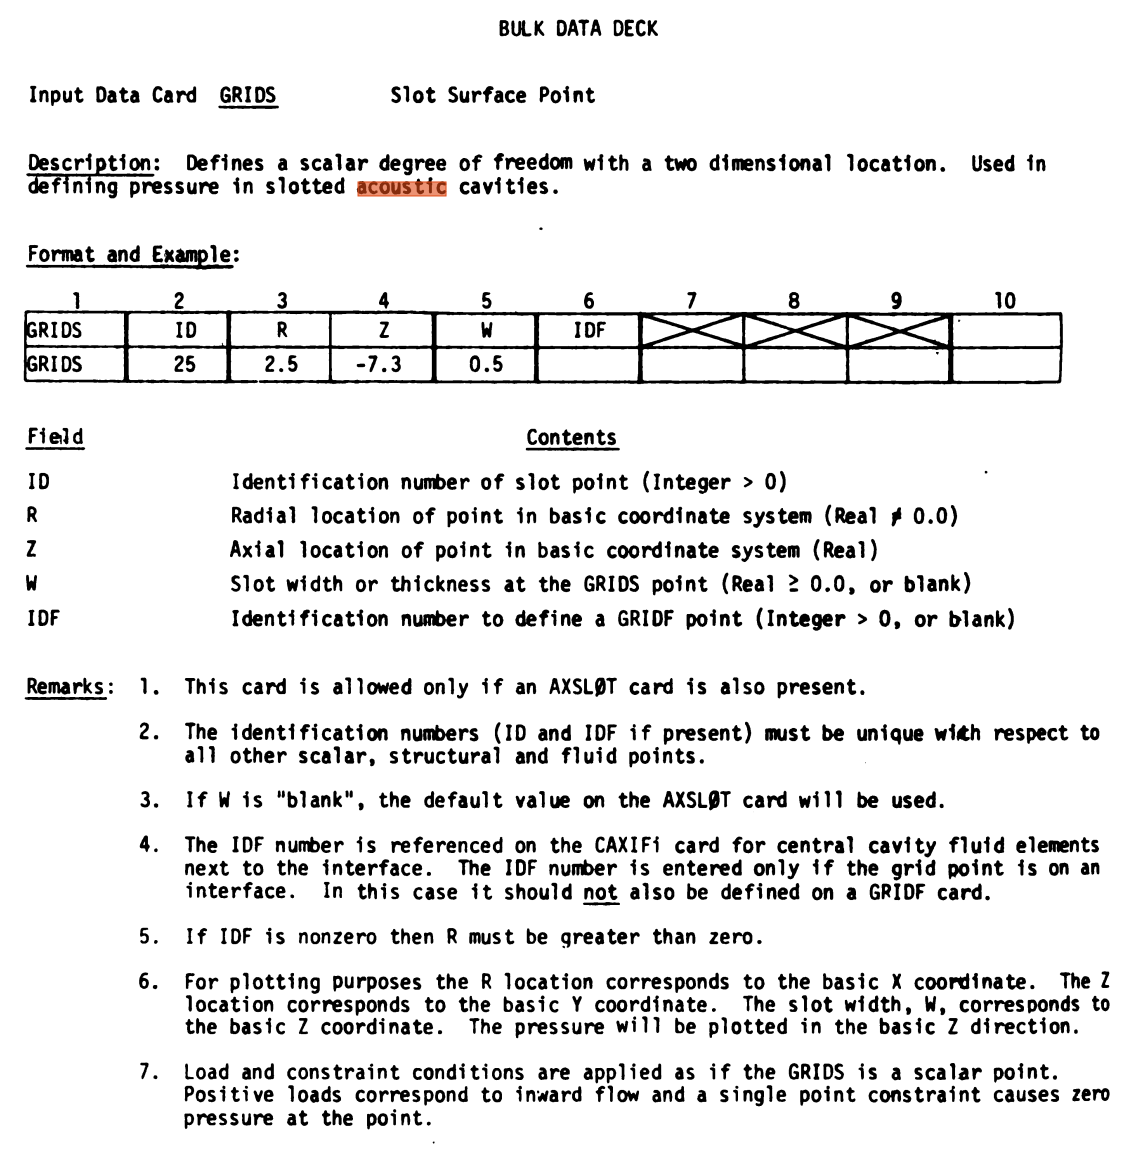
\includegraphics[scale=0.35]{nastran_fig9}
%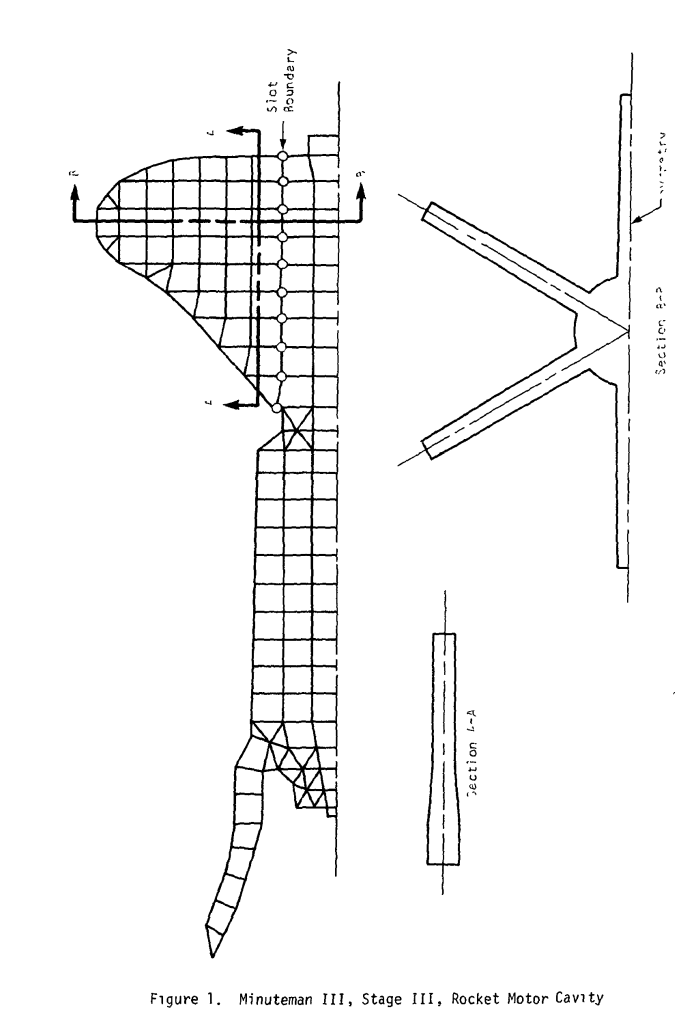
\includegraphics[width=3cm,height=5cm]{nastran_fig1}
    \caption{acoustic axisymmetric cavity analysis}
\end{figure}

\begin{figure}[h]
    \centering
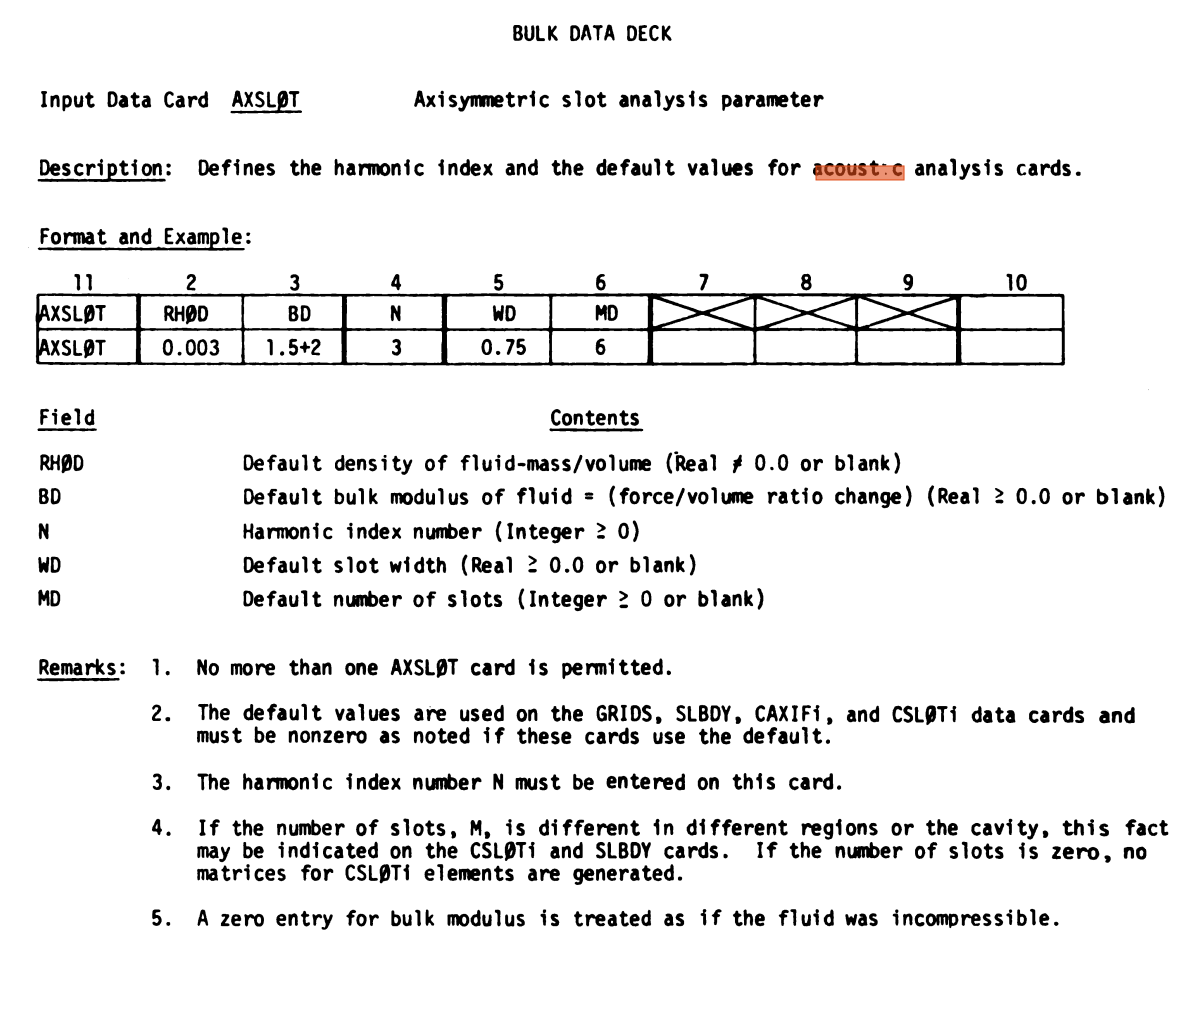
\includegraphics[scale=0.35]{nastran_fig10}
%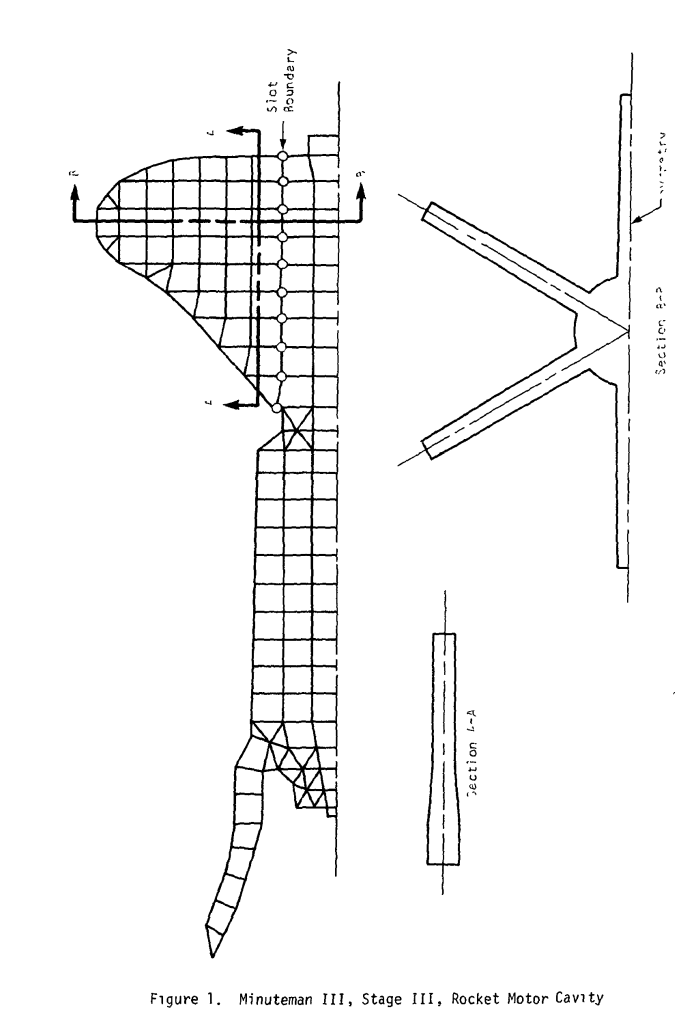
\includegraphics[width=3cm,height=5cm]{nastran_fig1}
    \caption{acoustic axisymmetric cavity analysis}
\end{figure}

\section{Acoustic CARDS}

\begin{itemize}

	\item AXSLOT Required to define existence of acoustic slot analysis, includes default parameters

	\item GRIDF Scalar degree of freedom for acoustic analysis of a fluid

	\item GRIDS Scalar degree of freedom on acoustic slot boundaries.

	\item CASIFi Fluid element connection i = 2, 3 or 4 fluid points in an acoustic slot analysis 
	\item CSLOTi Defines an element connecting i = 3 or i = 4 points which solves the wave equation
in two dimensions . Used in the acoustic cavity analysis for the definition of evenly spaced
radial slots 
\end{itemize}


\section{Supplement - Acoustic cavity modeling}

\subsection{1.9.1 - Data Card Functions}

The NASTRAN structural analysis system is used as the basis for acoustic cavity analysis .
Many of the structural analysis options such as selecting boundary conditions, applying loading
conditions, and selecting output data are also available for acoustics.
The data cards specifically used for acoustic cavity analysis are described below . The card
formats are exhibited in Section 2 . 4 . Their purposes are analogous to the use of structural data
cards . A gridwork of points is distributed over the longitudinal cross section of an acoustic
cavity and finite elements are connected between these points to define the enclosed volume.
The points are defined by GRIDF data cards for the axisymmetric central fluid cavity and by
GRIDS data cards for the radial slots. The GRIDF points are interconnected by finite elements via
the CAXIF2 , CAXIF3, and CAXIF4 data cards to define a cross sectional area of the body of rotation .
The CAXIF2 element data card defines the area
area of the cross section between the axis and two points
ross
S
off the axis (the GRIDF points may not have a zero radius) . The CAXIF3 and CAXIF4 data cards define
triangular or quadrilateral cross sections and connect three or four GRIDF points respectively.
The density and/or bulk modulus at each location of the enclosed fluid may also be defined on these
cards .
The GRIDS points in the slot region are interconnected by finite elements via the CSLØT3 and
CSLØT4 data cards .
These define finite elements with triangular and quadrilateral cross -sectional
shapes respectively. The width of the slot and the number of slots may be defined by default
values on the AXSLØT data card .
If the width of the slots is a variable , the value is specified
on the GRIDS cards at each point . The number of slots , the density, and /or the bulk modulus of
the fluid may also be defined individually , for each element on the CSLØT3 and CSLØT4 cards .
The AXSLØT data card is used to define the overall parameters for the system . Some of these
parameters are called the " default" values and may be selectively changed at particular cross
sections of the structure. The values given on the AXSLØT card will be used if a corresponding
value on the GRIDS , CAXIFI, or CSLØTi is left blank. The parameters o (density) and B ibulk
modulus ) are properties of the fluid .
If the value given for Bulk Modulus is zero the fluid is
considered incompressible to the program . The parameters M (Number of slots ) and W (slot width )
are properties of the geometry. The parameter M defines the number of equally spaced slots
around the circumference with the first slot located at 0 = 0° . The parameter N (harmonic number )
is selected by the user to analyze a particular set of acoustic modes.
The pressure is assumed
to have the following distribution
plr,2 ,0) = plr ,z ) cos No
If N = 0 the breathing and longitudinal modes will result.
If N = 1 the pressure at 0 = 180°
will be the negative of the pressure at 0 = 0°. If N = 2 , the pressures at 0 = 90° and 0 = 270o
will be the negative of that at 0 = 0°. Values of N larger than M / 2 have no significance.
The interface between the central cavity and the slots is defined with the SLBDY data cards .
The data for each card consists of the density of the fluid at the interface , the number of radial
slots around the circumference , and a list of GRIDS points that are listed in the sequence in
which they occur as the boundary is traversed . In order to ensure continuity between GRIDF and
GRIDS points at the interface , the GRIDF points on the boundary between the cylindrical cavity
and the slots are identified on the corresponding GRIDS data cards rather than on GRIDF cards.
Thus, the locations of the GRIDF points will be exactly the same as the locations of the corre
sponding GRIDS points.
Various standard NASTRAN data cards may be used for special purposes in acoustic analysis.
The SPCI data card may be used to constrain the pressures to zero at specified points such as at
a free boundary . The formats for these cards are included in Section 2 .4 . Dynamic load cards ,
direct input matrices , and scalar elements may be introduced to account for special effects.
The
reader is referred to Sections 1 . 4 and 1 . 5 for instruction in the use of these cards

\subsection{1.9.2 - Assumptions and limitations}

The accuracy of the acoustic model will be dependent on the selection of the mesh of finite
elements.
The assumption for each element is that the pressure field has a linear variation over
the cross section and a sinusoidal variation around the axis in the circumferential direction . In
areas where the pressure gradient changes are large, such as near a sharp corner , the points in
the mesh should be placed closer together so that large changes in flow may be defined accurately
by the finite elements.
The shape of the finite elements play an important part in the accuracy of the results .
It
has been observed that long narrow elements produce disproportionate errors. Cutting a large 
square into two rectangles will not improve the results whereas dividing the square into four
smaller squares may decrease the local error by as much as a factor of ten .
The slot portion of the cavity is limited to certain shapes because of basic assumptions in
the algorithms.
The cross section of the cavity normal to the axis must have a shape that is
reasonably well defined by a central circular cavity having equally spaced, narrow slots . Various
shapes are shown in Figure 1 in the order of increasing expected error.
It is recommended that shapes such as the cloverleaf and square cross section be analyzed
with a full three dimensional technique . The assumption of negligible pressure gradient in the
circumferential direction within a slot is not valid in these cases.
The harmonic orders of the solutions are also limited by the width of the slots. The
harmonic number, N , should be no greater than the number of slots divided by two .
The response
of the higher harmonics is approximated by the slot width correction terms discussed in the
NASTRAN Theoretical Manual, Section 17 .1.
The output data for the acoustic analysis consists of the values of pressure in the displace
ment vector selected via the case control card " PRESSURE = j" . The velocity vector components
corresponding to each mode may be optionally requested by the case control card "STRESS = i" ,
where i is the set number indicating the element numbers to be used for output , or by the words
" STRESS = ALL" .
The " SET =" card lists the element or point numbers to be output.
Plots of the finite element model and /or of the pressure field may be requested with the
NASTRAN plot request data cards.
The central cavity cross section will be positioned in the XY
plane of the Basic Coordinate System of NASTRAN. The slot elements are offset from the XY plane
by the width of the slot in the + z direction . The radial direction corresponds to X and the
axial direction corresponds to the y direction . Pressures will be plotted in the Z direction for
both the slot points and the central cavity points . The case control data cards for plotting are
documented in the User 's Manual. The PLOTEL elements are used for plotting the acoustic cavity
shape. The plot request card "SET n INCLUDE PLØTEL" must be used where n is a set number

\subsection{1.9.3 Acoustic Cavity Example Problem}

Table 1 contains a listing of the data cards used as a simple example of acoustic cavity
analysis. The problem to be solved is illustrated in Figure 2. The model was subdivided into
only ten finite elements in order to limit the number of data cards . For reasonable engineering
accuracy , this model should be subdivided into at least four times that number of elements .
Each data card in Table 1 is given a number on the left side .
The format for each type of
bulk data card is given in parentheses above the group of that type . The following is a brief
description of each card:

\begin{itemize}
	\item 1- 5
Each data card in the Executive Control deck has the format of a request word and a
selection separated by blanks or a comma . The ID card is first, the CEND card is last ,
but the intermediate cards may appear in any order . The user may put any pair of words
on the ID card for identification purposes. In this particular case Rigid Format
number 3 ( SØL 3 ,0 ) was chosen which is Normal Modes analysis. A limit of 2 minutes
CPU time was set (TIME 2 )
	\item 6 -7:  The TITLE = and SUBTITLE = cards may contain any list of letters and numbers following the
(=) sign . This list will appear on the first two lines of each output page
	\item 8: The method of eigenvalue extraction is selected with the METHØD = data card .
The number
11 refers to the identification number of an EIGR bulk data card which appears below as
card 32 and 33.
	\item 9 -11 A simple output request is illustrated with these cards. PRES= ALL will result in print
out of all pressures at the GRIDF and GRIDS points .
STRESS =ALL will result in the print
out of all velocities in the elements . This printout will occur for all extracted eigen
vectors. Selected points or elements can be printed via the SET card described in the
User ' s Manual .
\item 12: The BEGIN BULK card denotes the beginning of the bulk data deck. The Bulk Data Deck
cards may occur in any order. Putting these cards in alphabetic sort will save NASTRAN
sorting time in large problems, however
\item 13: In this problem all the parameters except slot width Wy are constant throughout the
volume.
The data values on the AXSLØT card will be used whenever a corresponding entry
in the following cards is blank
\item 21, 22:
The location of points within the axisymmetric fluid cavity are described by the GRIDF
card. No points are allowed to have a zero or negative radius .
\item 23-31:
These cards describe the elements shown in Figure 2 . Each element is given a unique
identification number and a list of the connected GRIDS or GRIDF points . Since the
parameters p and B are constants, these fields are left blank so the values on the AXSLØT
card will be used
\item 32 , 33 :
The EIGR card is used to define parameters for eigenvalue extraction (resonant frequen
cies) . More than one of these cards may appear.
The method to be used is selected with
the METHOD= data card in the Case Control Deck (card 8 ). With this particular card we
selected the Givens Tridiagonalization method (GIV) with a desired number of three
(Nd = 3) output mode shapes . The modes will be normalized such that the maximum pressure
is 1 .0 (NØRM =MAX) .These two cards illustrate a continuation card
\item 34: The SLBDY card defines the boundary between the slot and the central cavity . Both the
density ( P) and the number of radial slots (M ) are blank so the AXSLØT defaults are used,
i. e. 0 = 1.2x10 ' and M = 4 . Only four GRIDS points are on the boundary so a continua
tion card is not necessary . Field 8 being blank signifies the last entry
\item 35: The ENDDATA card is required to denote the end of the bulk data. Any following cards will
be ignored by NASTRAN
\item
\end{itemize}

\end{document}
